\chapter{Wprowadzenie}

Inspiracje biologiczne są obecne w~inżynierii już od wielu lat. Możemy się na nie natknąć nie tylko w~mechanice, awionice czy rbotyce. Zagrzały one miejsce również wśród szeroko rozumianych metod sztucznej inteligencji (ang. \textit{Artificial Intelligence, AI}). Jedną z~najciekawszych inspiracji na tym polu wydają sie być sztuczne sieci neuronowe (ang. \textit{Artificial Neural Networks, ANN}). Ich koncepcja pojawiła się już w połowie XX wieku \cite{perceptron}, jednak brak teoretycznych podstaw, które umożliwiałyby efektywne uczenie sieci sprawi, że nie zyskały one popularności w~następnych latach. Dopiero zaproponowana w~1986 metoda wstecznej propagacji błędu \cite{backprop} spowodowała powrót do koncepcji ANN szerszego grona badaczy. Dynamiczny wzrost mocy obliczeniowej komputerów oraz wypracowanie solidnych podstaw teoretycznych sprawiły, że sztuczne sieci neuronowe są dzisiaj jednym z~głównych narzędzi sztucznej inteligencji, które wykorzystywane jest w~badaniach naukowych, analizach rynku czy szeroko pojętym modelowaniu.

\section*{Opis projektu}

Chociaż algorytmy oparte na wstecznej propagacji błędu stanowiły przez lata oś zainteresowania w~kwestii uczenia ANN okazują się one nie być jedynymi dostępnymi. Celem naszego projektu było zaimplementowanie alternatywnych metod uczenia opartych o~mechanizmy znane z~algorytmów ewolucyjnych, sprawdzenie ich wydajności oraz porównanie z podejściem klasycznym na bazie gier znanych z~konsoli Atari. Jako środowisko testowe posłużyła nam otwarta biblioteka \textit{OpenAI Gym} dostępna w języku Python. Poprzez prosty interfejs udostępnia ona szerek ujednoliconych środowisk testowych umożliwiających testowanie algorytmów uczenia ze wzmocnieniem. Spośród nich wybraliśmy emulację gry Breakout (w~wersji ze stanem reprezentowanym przez pamięć RAM gry).  Klasyczne wykorzystanie sieci neuronowych kojarzy się raczej z~uczeniem nadzorowanym, którego zadaniem jest budowa modelu potrafiącego przypisać danym wejsciowym jedną z~dostępnych etykiet. Istnieją jednak metody uczenia, które pozwalają wykorzystać sieci równiez w~zadaniach uczenia ze wzmocnieniem. Właśnie jedeną z takich metod - \textit{Deep Q Learning} - wykorzystaliśmy jako punkt odniesienia dla podejścia ewolucyjnego.

\begin{figure}
    \centering
    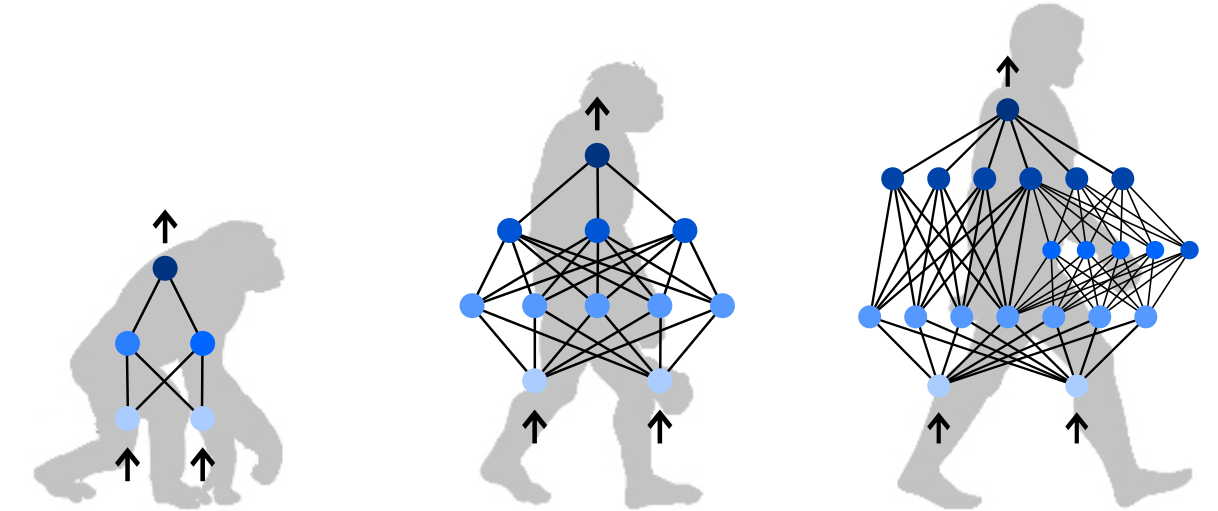
\includegraphics[scale=0.3]{neuroevolution.png}
    \caption{Poglądowe spojrzenie na neuroewolucję}
    \label{neuroevolution}
\end{figure}

Jednym z~największych problemów stojących przed projektantem sztucznej sieci neuronowej jest odpowiedni dobór hiperparametrów takich jak ilość wartw czy ilość neuronów w~poszczególnych warstwach. Dzięki wykorzystaniu mechanizmów ewolucyjnych możliwe jest stworzenie algorytmów, które poza parametrami sieci dostosowują również w~dynamiczny sposób jej topologię. W~ramach projektu zdecydowaliśmy się zbadać zarówno metody o~stałej jak i~o~zmiennej topologii co dobprowadziło do wyróżnienia czterech rónych wariantów uczenia:

\vskip 0.5cm
\begin{itemize}[leftmargin=1cm]
    \item[$\bullet$] uczenie sieci o~stałej topologii z~wykorzystaniem wstecznej propagacji błędu
    \item[$\bullet$] uczenie sieci o~stałej topologii z~wykorzystaniem algorytmu ewolucyjnego
    \item[$\bullet$] uczenie sieci o~zmiennej topologii dostosowywanej przez algorytm ewolucyjny; dobór wag metodą wstecznej propagacji błędu
    \item[$\bullet$] uczenie sieci o~zmiennej topologii dostosowywanej przez algorytm ewolucyjny; dobór wag metodą ewolucyjną
\end{itemize}
\vskip 0.5cm